\documentclass[paper=a4, fontsize=11pt]{article} 

\usepackage[T1]{fontenc} 

\usepackage[utf8]{inputenc}
\usepackage[francais]{babel} 
\usepackage{mathtools}
\usepackage{amssymb}
\usepackage{alltt}
\usepackage{float}
\usepackage{graphicx}
\usepackage[colorinlistoftodos]{todonotes}
\usepackage{geometry}
\usepackage{hyperref}
\usepackage{enumitem}

\title{\normalfont \normalsize 
\huge TP 2 - Problèmes sous contraintes et algorithmes associés}

\author{Jules Kozolinsky}

\date{}

\begin{document}
\maketitle
\section{Optimisation sous contraintes égalités - Lagrangien augmenté}
\subsection{Solution analytique du problème}
Le problème est le suivant : 
\begin{align*}
\text{min}_{u \in U} J(u) := u_1 + u_2 
\end{align*}
où 
\begin{align*}
U = \lbrace u = (u_1,u_2) \in \mathbb{R}^2 / \varphi(u) = u_1^2 + u_2^2 -2 = 0 \rbrace
\end{align*}
Introduisons le lagrangien :
\begin{align*}
\mathcal{L}(u,\lambda) = J(u) + \lambda\varphi(u)
\end{align*}
On a alors : 
\begin{align*}
\nabla_u \mathcal{L} = 1 + 2\lambda u 
\end{align*}
Ainsi, comme $\lambda \in \mathbb{R}, u_1 = u_2$.\\
Puis comme $\varphi(u) = 0$, on a $u_1 = 1$ ou $u_1 = -1$. \\
Donc, pour obtenir le minimum, il faut $u_1 = u_2 = -1$ pour lequel on obtient $J(u) = -2$.
\subsection{Résolution numérique}
Pour une précision de $10^{-8}$, on obtient une solution en $17$ itérations seulement. (cf Figure \ref{étiquette1})
\begin{figure}
 	\begin{center}
   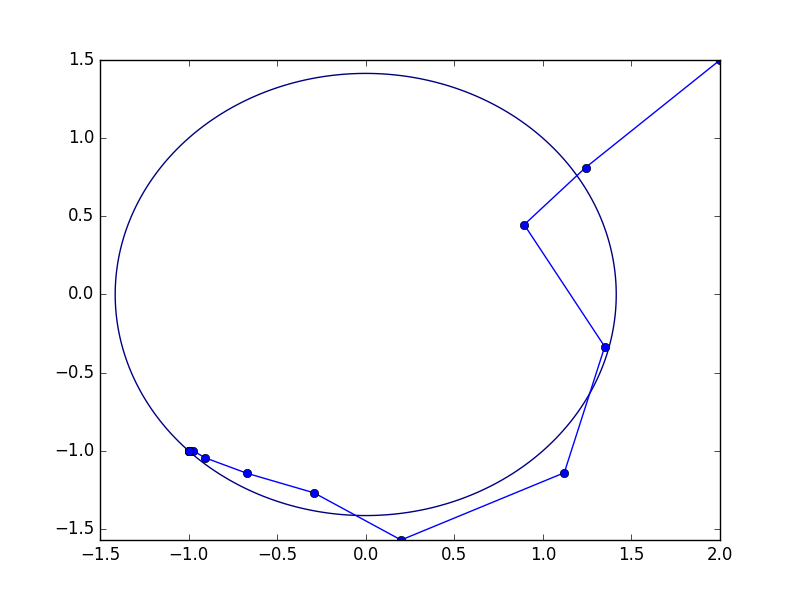
\includegraphics[scale=0.6]{lagrangien-augmente}
   \end{center}
   \caption{\label{étiquette1} Itérés $u_k$ et contrainte $U$ }
\end{figure}

\section{Problème d'élasticité en contact. Algorithme d'Uzawa}
L'algorithme d'Uzawa est très efficace pour résoudre ce problème.
\subsection{$f=0$}
Pour $f=0$, avec une précision de $10^{-6}$, on obtient une solution en $1292$ itérations.(cf Figure \ref{étiquette2})
\begin{figure}
 	\begin{center}
   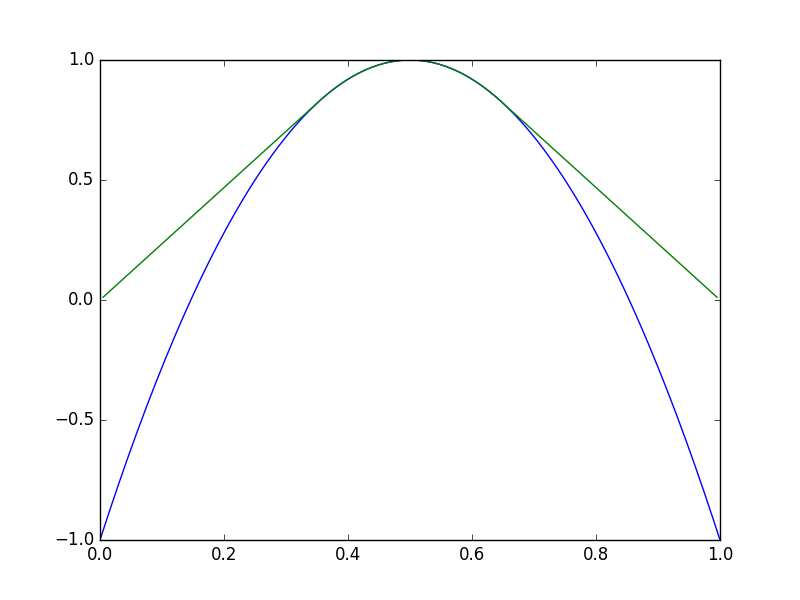
\includegraphics[scale=0.6]{uzawa_0}
   \end{center}
   \caption{\label{étiquette2} Membrane élastique pour $f=0$ }
\end{figure}
\subsection{$f=-100$}
Pour $f=-100$, avec une précision de $10^{-6}$, on obtient une solution en $1672$ itérations. (cf Figure \ref{étiquette3})
\begin{figure}
 	\begin{center}
   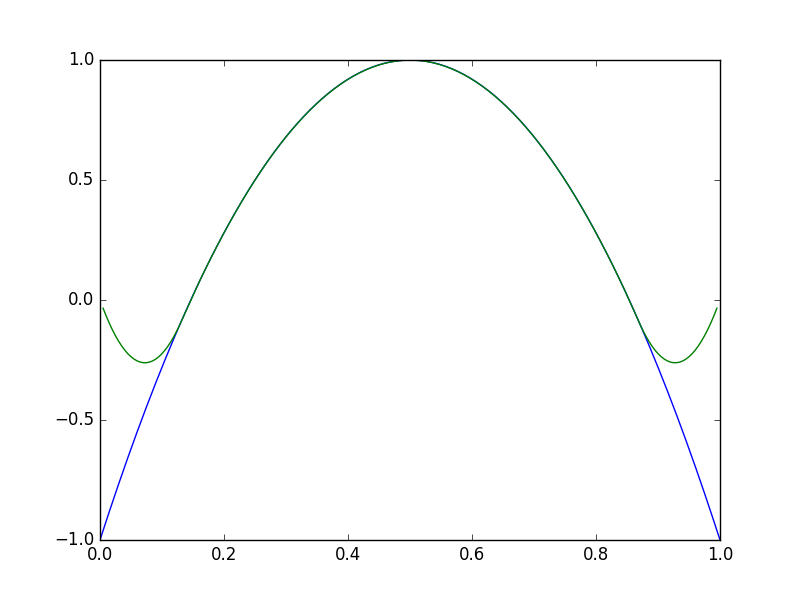
\includegraphics[scale=0.6]{uzawa_-100}
   \end{center}
   \caption{\label{étiquette3} Membrane élastique pour $f=-100$ }
\end{figure}

\section{Conformation atomique d'une nano-particule et potentiel de Lennard-Jones}
\subsection{Résolution analytique et numérique $N=4$}
\subsubsection{Solution théorique}
On pose 
\begin{align*}
X_1 &= 0 \\
X_2 &= (x_2,0,0)^T\\
X_3 &= (x_3,y_3,0)^T\\
X_4 &= (x_4,y_4,z_4)^T\\
\end{align*}
Et $J(X_1,X_2,X_3,X_4) = V(r_{12}) + V(r_{13}) + V(r_{14}) + V(r_{23}) + V(r_{24}) + V(r_{34})$.
Or 
\begin{align*}
d_{12} = r_{12}^2 &= ||X_1 - X_2||^2 = x_2^2\\
d_{13} = r_{13}^2 &= ||X_1 - X_3||^2 = x_3^2 + y_3^2\\
d_{14} = r_{14}^2 &= ||X_1 - X_4||^2 = x_4^2 + y_4^2 + z_4^2\\
d_{23} = r_{23}^2 &= ||X_2 - X_3||^2 = (x_2-x_3)^2 + y_3^2\\
d_{24} = r_{24}^2 &= ||X_1 - X_4||^2 = (x_2-x_4)^2 + y_4^2 + z_4^2\\
d_{34} = r_{34}^2 &= ||X_1 - X_4||^2 = (x_3-x_4)^2 + (y_3-y_4)^2 + z_4^2\\
\end{align*}
et, en remplaçant $r$ par $d=r^2$, on renomme $V$ et $U$ pour simplifier les calculs de dérivés :
\begin{align*}
U(d) &= \frac{1}{d^6} - \frac{2}{d^3}\\
U'(d) &= \frac{6}{d^4}(1-\frac{1}{d^3})
\end{align*}
D'où $J(X_1,X_2,X_3,X_4) = U(d_{12}) + U(d_{13}) + U(d_{14}) + U(d_{23}) + U(d_{24}) + U(d_{34})$.
Ainsi, par annulation des gradients, on a : $d_{34} = d_{24} = d_{23} = d_{14} = d_{13} = d_{12} = 1$.
Ainsi, on trouve : 
\begin{align*}
&x_2^2 = 1 \\
&x_3 = \text{sign}(x_2)\frac{1}{2}\\
&x_3 = x_4\\
&y_3^2 = \frac{3}{4}\\
&y_4 = \text{sign}(y_3)\frac{1}{3}\\
&z_4^2 = \frac{23}{36} 
\end{align*}
Ainsi, l'ensemble des solutions est de cardinal $8$.
\subsubsection{Résolution numérique}
On initialise avec un vecteur aléatoire. 
On obtient un valeur minimale de $J_4 = -6.0$ avec une précision de $10^{-7}$ en $10^3$ itérations en moyenne. \\
L'énergie minimum des atomes est donc représentée sous un simplexe de dimension $4$.\\
On obtient $X_1 = 0$ (fixé), $X_2 = (-1,0,0)$, $X_3 = (-0.5,-0.86,0)$ et $X_4 = (-0.5,-0.29,0.81)$.\\
(On est proche des valeurs théoriques)

\begin{figure}
 	\begin{center}
   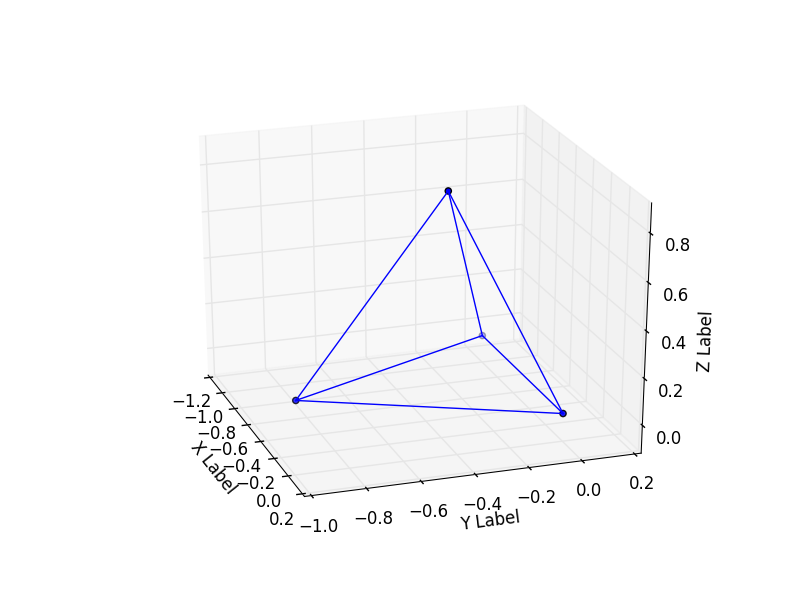
\includegraphics[scale=0.6]{atoms_4}
   \end{center}
   \caption{\label{étiquette4} $(X_1,X_2,X_3,X_4)$ optimum}
\end{figure}

\subsection{Résolution numérique pour $N=13$}
On initialise également avec un vecteur aléatoire. 
On obtient un palier de convergence pour $J_N = -36.3$ (cf Figure \ref{étiquette5} et \ref{étiquette6} ).\\
Pourtant dans la littérature (sujet de l'agreg), on trouve un minimum d'environ $-44$.
En effet, on n'a pas exactement un icosaèdre régulier.
Cela est peut-être dû à la mauvaise initialisation choisie ici, mais je n'en trouve pas de mieux. 
\begin{figure}
 	\begin{center}
   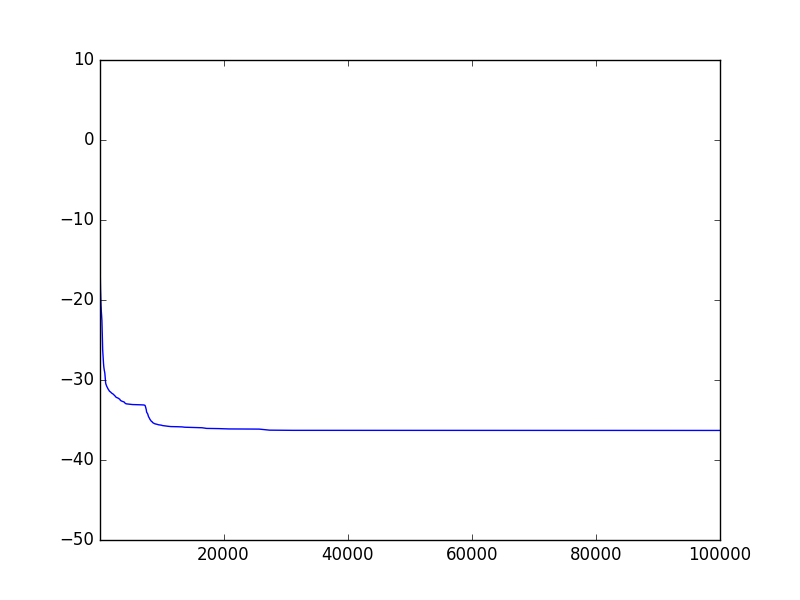
\includegraphics[scale=0.6]{convergence}
   \end{center}
   \caption{\label{étiquette5} Historique de convergence de J}
\end{figure}
\begin{figure}
 	\begin{center}
   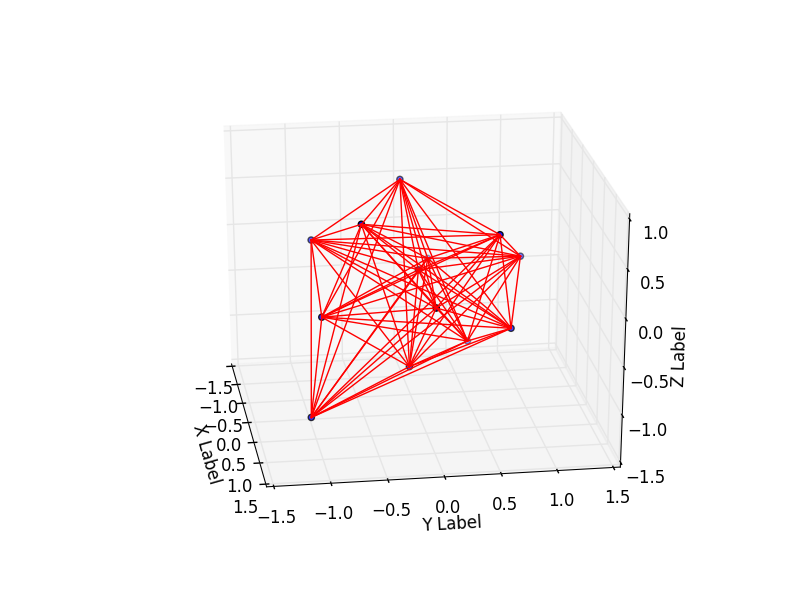
\includegraphics[scale=0.6]{icosaedre}
   \end{center}
   \caption{\label{étiquette6} Solution optimale}
\end{figure}

\end{document}